%!TEX root=../protocol.tex	% Optional

\section{Lösung}

\subsection{ActiveMQ}

\subsubsection{Allgemein}

Für die Message Oriented Middleware verwende ich \textbf{ActiveMQ}, ein open source 'Message Broker' von Apache.

Der neueste Build ist zum Download verfügbar auf der \href{http://activemq.apache.org/download.html}{ActiveMQ Download Seite}, in meinem Fall ist das \textbf{ActiveMQ 5.15.3 (Unix/Linux)}.

\subsubsection{Installieren}

Ich habe mir ActiveMQ als soft-link hinzugefügt, sodass ich es von überall aufrufen kann:

\begin{code}{shell}
$ tar -xzf apache-activemq-5.15.3-bin.tar.gz
$ mv apache-activemq-5.15.3-bin ~/activemq
$ cd ~/activemq/bin
$ chmod +x activemq
$ sudo ln -s /home/mrousavy/activemq/bin/activemq /usr/bin/activemq
$ activemq start
\end{code}

Nun ist der \textbf{ActiveMQ} Apache server unter \url{http://localhost:8161/admin} erreichbar. Benutzername und Passwort sind standardmäßig \texttt{admin} und \texttt{admin}.

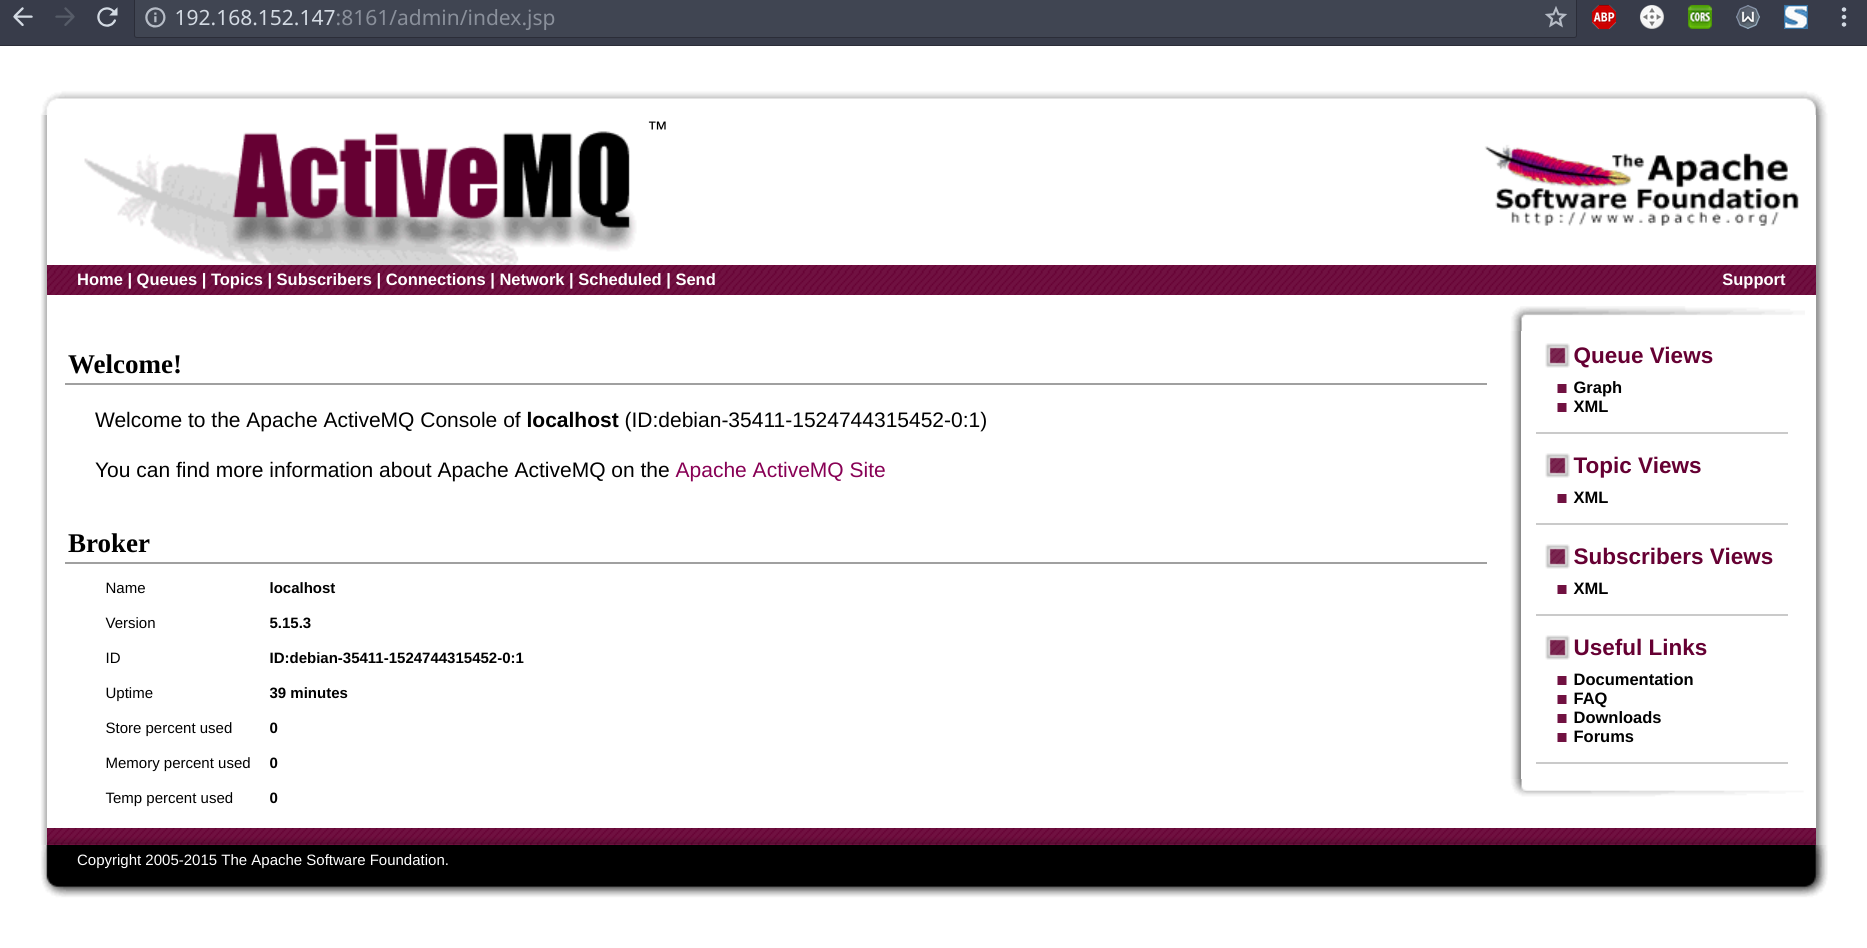
\includegraphics[width=\textwidth]{images/activemq-home}

Der Status des ActiveMQ services kann mittels

\begin{code}{shell}
$ activemq status
\end{code}

abgerufen werden.

\subsubsection{Java}

Als nächstes muss ein Java Projekt erstellt werden, wozu ich \textbf{IntelliJ IDEA} verwende.

Nun muss die \textbf{ActiveMQ} library zu dem Projekt hinzugefügt werden, hierbei wird die library \texttt{activemq-all-5.15.3.jar} bereits in dem \texttt{apache-activemq-5.15.3-bin.tar.gz} archiv mitgegeben, jedoch verwende ich \textbf{Maven} um den Prozess der Libraries zu vereinfachen.

Die \textbf{ActiveMQ} library ist mittels folgendem \texttt{dependency} tag in dem \texttt{pom.xml} file hinzuzufügen:

\begin{code}{xml}
<dependencies>
    <dependency>
        <groupId>org.apache.activemq</groupId>
        <artifactId>activemq-all</artifactId>
        <version>5.8.0</version>
    </dependency>
</dependencies>
\end{code}

Ich verwende das Package \texttt{activemq-all}, da hier alle Artifakte inkludiert sind (\texttt{activemq-core}, ..).

\clearpage




\subsection{Windfarm}

Für eine \textbf{Windfarm} benötigen wir ein individuelles Windrad~\ref{sec:windmill} welches Daten misst, einen Windpark~\ref{sec:windfarm} welcher Daten aller Windräder misst und eine Zentrale~\ref{sec:headquarters} welche die Daten aller Windparks misst.

\subsubsection{Windrad}
\label{sec:windmill}

Das Windrad (\textit{Windmill}) benötigt eine ID sowie eine Referenz zu dem Windpark (\textit{Windfarm}).

Es soll die Windgeschwindigkeit, die Rotationsgeschwindigkeit, die Einheit der Geschwindigkeit, den Strom-output, die Einheit des Strom-outputs, die Blatt-position und die Latenz messen.

Außerdem wäre es hilfreich einen Zeitstempel mitzuspeichern.

Die Implementation folgt in der Klasse \texttt{Windmill.java}:

\begin{code}{java}
// Windmill.java

@XmlRootElement
public class Windmill {
    @XmlTransient
    public Windfarm farm = null;
    @XmlElement
    public int id = 0;
    @XmlElement
    public double windSpeed = 0.0;
    @XmlElement
    public SpeedUnit speedUnit = SpeedUnit.KMH;
    @XmlElement
    public double powerOutput = 0.0;
    @XmlElement
    public PowerUnit powerUnit = PowerUnit.MEGA_WATT;
    @XmlElement
    public double rotationSpeed;
    @XmlElement
    public double bladePosition;
    @XmlElement
    public double latency;

    @XmlElement(name = "timestamp")
    public String getTimestamp() {
        DateFormat dateFormat = new SimpleDateFormat("dd.MM.yyyy HH:mm:ss");
        return dateFormat.format(new Date());
    }
}
\end{code}

Wobei die \texttt{Enum}s folgendermaßen definiert sind:

\begin{code}{java}
// Windmill.java

// Measurement of Speed
public enum SpeedUnit {
    KMH,
    MPH
}

// Measurement of Power
public enum PowerUnit {
    KILO_WATT,
    MEGA_WATT,
    GIGA_WATT
}
\end{code}

Um das ganze zu einem XML zu \textit{parsen}, habe ich folgende Methode geschrieben:

\begin{code}{java}
    // Windmill.java

    public String buildXml() {
        try {
            JAXBContext jaxbContext = JAXBContext.newInstance(Windmill.class);
            Marshaller jaxbMarshaller = jaxbContext.createMarshaller();
            jaxbMarshaller.setProperty(Marshaller.JAXB_FORMATTED_OUTPUT, true);
            StringWriter sw = new StringWriter();
            jaxbMarshaller.marshal(this, sw);
            return sw.toString();
        } catch (JAXBException e) {
            e.printStackTrace();
            return "";
        }
    }
\end{code}

\clearpage
\subsubsection{Windpark}
\label{sec:windfarm}

Der Windpark (\textit{Windfarm}) benötigt eine ID sowie eine Liste aus Windrädern.

Die Implementation folgt in der Klasse \texttt{Windfarm.java}:

\begin{code}{java}
// Windfarm.java

@XmlRootElement
public class Windfarm {
    @XmlElement
    public int id = 0;
    @XmlElement(name = "windmill")
    public ArrayList<Windmill> mills = new ArrayList<Windmill>();
}
\end{code}

\

Außerdem habe ich folgende Methode geschrieben um die Windfarm zu XML zu \textit{parsen}:

\begin{code}{java}
    // Windfarm.java

    public String buildXml() {
        try {
            JAXBContext jaxbContext = JAXBContext.newInstance(Windfarm.class);
            Marshaller jaxbMarshaller = jaxbContext.createMarshaller();
            jaxbMarshaller.setProperty(Marshaller.JAXB_FORMATTED_OUTPUT, true);
            StringWriter sw = new StringWriter();
            jaxbMarshaller.marshal(this, sw);
            return sw.toString();
        } catch (JAXBException e) {
            e.printStackTrace();
            return "";
        }
    }
\end{code}

\

Diese Klasse soll in der Lage sein, mit der Middleware (ActiveMQ) zu kommunizieren. Hierzu werden folgende Attribute benötigt:

\begin{code}{java}
// Windfarm.java

@XmlTransient
private Session session = null;
@XmlTransient
private Connection connection = null;
@XmlTransient
private MessageProducer producer = null;
\end{code}

Sie wurden als \texttt{@XmlTransient} markiert, weil sie von der \texttt{buildXml} Methode (und somit dem \texttt{Marshaller}) nicht erfasst und \textit{geparsed} werden sollen.

Für die Herstellung einer Verbindung zu dem \textbf{ActiveMQ} Service habe ich folgende Methode implementiert:

\begin{code}{java}
// Windfarm.java

public void connect() throws JMSException {
    ActiveMQConnectionFactory factory = new ActiveMQConnectionFactory(Statics.USER, Statics.PASSWORD, Statics.URL);
    connection = factory.createConnection();
    connection.start();

    // Create the session
    session = connection.createSession(false, Session.AUTO_ACKNOWLEDGE);
    Destination destination = session.createTopic(Statics.SUBJECT);

    // Create the producer.
    producer = session.createProducer(destination);
    producer.setDeliveryMode(DeliveryMode.NON_PERSISTENT);
}
\end{code}

..sowie folgende Methode zum senden der derzeitigen Werte:

\begin{code}{java}
// Windfarm.java

public void send() throws JMSException {
    TextMessage message = session.createTextMessage(buildXml());
    System.out.println(message.getText());
    producer.send(message);
}
\end{code}

..und folgende Methode zum stoppen und schließen der Verbindung:

\begin{code}{java}
// Windfarm.java

public void stop() throws JMSException {
    connection.close();
    producer.close();
    session.close();
}
\end{code}

\

Um das ganze zu testen, bastelte ich schnell diese Main Methode zusammen, welche jede halbe Sekunde das derzeitige XML an die \gls{mom} schickt:

\begin{code}{java}
// Windfarm.java

public static void main(String[] args) {
    try {
        System.out.println("Starting Windfarm..");

        Windfarm farm = new Windfarm();
        farm.connect();
        // send XML every half second, 10 times
        for (int i = 0; i < 10; i++) {
            System.out.println("Sending XML..");
            farm.send();
            Thread.sleep(500);
        }
        // stop service
        farm.stop();

        System.out.println("Windfarm finished!");
    } catch (JMSException ex) {
        System.out.println("[Windfarm] error: " + ex);
        ex.printStackTrace();
    } catch (InterruptedException e) {
        e.printStackTrace();
    }
}
\end{code}

\clearpage
\subsubsection{Zentrale}
\label{sec:headquarters}

Die Zentrale (\textit{Headquarter}) soll lediglich die Daten von der \gls{mom} auslesen und anzeigen.

Die Implementation folgt in der \texttt{Headquarter.java} Datei.

Es wird wieder eine Methode zum Verbinden benötigt:

\begin{code}{java}
// Headquarter.java

public void connect() throws JMSException {
    ActiveMQConnectionFactory factory = new ActiveMQConnectionFactory(Statics.USER, Statics.PASSWORD, Statics.URL);
    connection = factory.createConnection();
    connection.start();

    // Create the session
    session = connection.createSession(false, Session.AUTO_ACKNOWLEDGE);
    Destination destination = session.createTopic(Statics.SUBJECT);

    // Create the consumer
    consumer = session.createConsumer(destination);
}
\end{code}

..sowie eine Methode zum empfangen bzw. auslesen von Messages:

\begin{code}{java}
// Headquarter.java

public void receive() throws JMSException {
    // Start receiving
    TextMessage message = (TextMessage) consumer.receive();
    if (message != null) {
        System.out.println("[Headquarter] Message received: " + message.getText());
        message.acknowledge();
    }
}
\end{code}

..und eine Methode zum beenden:

\begin{code}{java}
// Headquarter.java

public void stop() throws JMSException {
    connection.close();
    consumer.close();
    session.close();
}
\end{code}

In diesem Beispiel werde ich den Headquarter-service starten um 10 Messages von der \gls{mom} auszulesen:

\begin{code}{java}
// Headquarter.java

public static void main(String[] args) {
    try {
        System.out.println("Starting Headquarter..");

        Headquarter hq = new Headquarter();
        hq.connect();
        // receive a message 10 times in total
        for (int i = 0; i < 10; i++) {
            hq.receive();
        }
        // stop the service
        hq.stop();

        System.out.println("Headquarter finished!");
    } catch (JMSException e) {
        e.printStackTrace();
    }
}
\end{code}
